\documentclass[journal,12pt,twocolumn]{IEEEtran}

\usepackage{setspace}
\usepackage{gensymb}
\singlespacing
\usepackage[cmex10]{amsmath}

\usepackage{amsthm}

\usepackage{mathrsfs}
\usepackage{txfonts}
\usepackage{stfloats}
\usepackage{bm}
\usepackage{cite}
\usepackage{cases}
\usepackage{subfig}

\usepackage{longtable}
\usepackage{multirow}

\usepackage{enumitem}
\usepackage{mathtools}
\usepackage{steinmetz}
\usepackage{tikz}
\usepackage{circuitikz}
\usepackage{verbatim}
\usepackage{tfrupee}
\usepackage[breaklinks=true]{hyperref}
\usepackage{graphicx}
\usepackage{tkz-euclide}

\usetikzlibrary{calc,math}
\usepackage{listings}
    \usepackage{color}                                            %%
    \usepackage{array}                                            %%
    \usepackage{longtable}                                        %%
    \usepackage{calc}                                             %%
    \usepackage{multirow}                                         %%
    \usepackage{hhline}                                           %%
    \usepackage{ifthen}                                           %%
    \usepackage{lscape}     
\usepackage{multicol}
\usepackage{chngcntr}

\DeclareMathOperator*{\Res}{Res}

\renewcommand\thesection{\arabic{section}}
\renewcommand\thesubsection{\thesection.\arabic{subsection}}
\renewcommand\thesubsubsection{\thesubsection.\arabic{subsubsection}}

\renewcommand\thesectiondis{\arabic{section}}
\renewcommand\thesubsectiondis{\thesectiondis.\arabic{subsection}}
\renewcommand\thesubsubsectiondis{\thesubsectiondis.\arabic{subsubsection}}


\hyphenation{op-tical net-works semi-conduc-tor}
\def\inputGnumericTable{}                                 %%

\lstset{
%language=C,
frame=single, 
breaklines=true,
columns=fullflexible
}
\begin{document}


\newtheorem{theorem}{Theorem}[section]
\newtheorem{problem}{Problem}
\newtheorem{proposition}{Proposition}[section]
\newtheorem{lemma}{Lemma}[section]
\newtheorem{corollary}[theorem]{Corollary}
\newtheorem{example}{Example}[section]
\newtheorem{definition}[problem]{Definition}

\newcommand{\BEQA}{\begin{eqnarray}}
\newcommand{\EEQA}{\end{eqnarray}}
\newcommand{\define}{\stackrel{\triangle}{=}}
\bibliographystyle{IEEEtran}
\raggedbottom
\setlength{\parindent}{0pt}
\providecommand{\mbf}{\mathbf}
\providecommand{\pr}[1]{\ensuremath{\Pr\left(#1\right)}}
\providecommand{\qfunc}[1]{\ensuremath{Q\left(#1\right)}}
\providecommand{\sbrak}[1]{\ensuremath{{}\left[#1\right]}}
\providecommand{\lsbrak}[1]{\ensuremath{{}\left[#1\right.}}
\providecommand{\rsbrak}[1]{\ensuremath{{}\left.#1\right]}}
\providecommand{\brak}[1]{\ensuremath{\left(#1\right)}}
\providecommand{\lbrak}[1]{\ensuremath{\left(#1\right.}}
\providecommand{\rbrak}[1]{\ensuremath{\left.#1\right)}}
\providecommand{\cbrak}[1]{\ensuremath{\left\{#1\right\}}}
\providecommand{\lcbrak}[1]{\ensuremath{\left\{#1\right.}}
\providecommand{\rcbrak}[1]{\ensuremath{\left.#1\right\}}}
\theoremstyle{remark}
\newtheorem{rem}{Remark}
\newcommand{\sgn}{\mathop{\mathrm{sgn}}}
\providecommand{\abs}[1]{\left\vert#1\right\vert}
\providecommand{\res}[1]{\Res\displaylimits_{#1}} 
\providecommand{\norm}[1]{\left\lVert#1\right\rVert}
%\providecommand{\norm}[1]{\lVert#1\rVert}
\providecommand{\mtx}[1]{\mathbf{#1}}
\providecommand{\mean}[1]{E\left[ #1 \right]}
\providecommand{\fourier}{\overset{\mathcal{F}}{ \rightleftharpoons}}
%\providecommand{\hilbert}{\overset{\mathcal{H}}{ \rightleftharpoons}}
\providecommand{\system}{\overset{\mathcal{H}}{ \longleftrightarrow}}
	%\newcommand{\solution}[2]{\textbf{Solution:}{#1}}
\newcommand{\solution}{\noindent \textbf{Solution: }}
\newcommand{\cosec}{\,\text{cosec}\,}
\providecommand{\dec}[2]{\ensuremath{\overset{#1}{\underset{#2}{\gtrless}}}}
\newcommand{\myvec}[1]{\ensuremath{\begin{pmatrix}#1\end{pmatrix}}}
\newcommand{\mydet}[1]{\ensuremath{\begin{vmatrix}#1\end{vmatrix}}}
\numberwithin{equation}{subsection}

\makeatletter
\@addtoreset{figure}{problem}
\makeatother
\let\StandardTheFigure\thefigure
\let\vec\mathbf

\renewcommand{\thefigure}{\theproblem}

\def\putbox#1#2#3{\makebox[0in][l]{\makebox[#1][l]{}\raisebox{\baselineskip}[0in][0in]{\raisebox{#2}[0in][0in]{#3}}}}
     \def\rightbox#1{\makebox[0in][r]{#1}}
     \def\centbox#1{\makebox[0in]{#1}}
     \def\topbox#1{\raisebox{-\baselineskip}[0in][0in]{#1}}
     \def\midbox#1{\raisebox{-0.5\baselineskip}[0in][0in]{#1}}
\vspace{3cm}
\title{Assignment 6}
\author{Sachinkumar Dubey - EE20MTECH11009}
\maketitle
\newpage
\bigskip
\renewcommand{\thefigure}{\theenumi}
\renewcommand{\thetable}{\theenumi}
Download all python codes from 
\begin{lstlisting}
https://github.com/sachinomdubey/Matrix-theory/Assignment6/codes
\end{lstlisting}
%
and latex-tikz codes from 
%
\begin{lstlisting}
https://github.com/sachinomdubey/Matrix-theory/Assignment6
\end{lstlisting}
\section{Problem}
(Rams 3.4.1) find the Asymptotes of the following:\\
\begin{align}
\vec{x}^T\myvec{1 & 0\\0 & -1}\vec{x}-\myvec{4 & 6}\vec{x}-6=0
\end{align}
\section{Explanation}
The following process is followed to get the equations of the Asymptotes:
\begin{enumerate}
    \item Move the origin to the center of the given equation to get equation of the form:
    \begin{align}
    \implies\vec{x}^T\vec{V}\vec{x}&=1 \label{eq2.0.1}
    \end{align}
    \item The equations of the Asymptotes of (\ref{eq2.0.1}) can be obtained by factoring the RHS and equating each factors to zero.
    \item Obtain the equations of the Asymptotes of the original equation by restoring the origin, which is done by replacing $\Vec{x}$ with $(\Vec{x}+\Vec{c})$ in the equations of the Asymptotes obtained in step2.
\end{enumerate}
\section{Solution}
Given,
\begin{align}
\vec{x}^T\myvec{1 & 0\\0 & -1}\vec{x}+2\myvec{-2 & -3}\vec{x}-6=0 \label{2.0.1}
\intertext{where,}
\vec{V}=\myvec{1 & 0 \\0 & -1}\\
\vec{u}=\myvec{-2 \\ -3}
\end{align}
Here, $ \det(\vec{V})=-1$. Since $\det(\vec{V})<0$ the given equation represents a hyperbola with center:
\begin{align}
\vec{c}&=-\vec{V}^{-1}\vec{u}=\myvec{2\\-3}
\end{align}
Moving the origin to the center $\vec{c}$, The above equation \eqref{2.0.1} can be modified as
\begin{align}
(\vec{x}+\vec{c})^T\vec{V}(\vec{x}+\vec{c})+2\vec{u}^T(\vec{x}+\vec{c})-6&=0\label{eq:solutions/3/4/1/finalsub}
\end{align}
From equation \eqref{eq:solutions/3/4/1/finalsub} consider,
\begin{align}
    &\implies(\vec{x}+\vec{c})^T\vec{V}(\vec{x}+\vec{c})\\
    &\implies\vec{x}^T\vec{V}\vec{x}+\vec{c}^T\vec{V}\vec{x}+\vec{x}^T\vec{V}\vec{c}+\vec{c}^T\vec{V}\vec{c}\label{eq:solutions/3/4/1/1n}\\
    \intertext{we know that}
    &\vec{x}^T\vec{V}\vec{c}=\vec{c}^T\vec{V}\vec{x}\label{eq:solutions/3/4/1/p}
    \intertext{Substituting equation \eqref{eq:solutions/3/4/1/p} in equation \eqref{eq:solutions/3/4/1/1n}}
    &\implies\vec{x}^T\vec{V}\vec{x}+2\vec{c}^T\vec{V}\vec{x}+\vec{c}^T\vec{V}\vec{c}\label{eq:solutions/3/4/1/eq1}
\end{align}
\begin{align}
    \vec{c}^T\vec{V}\vec{x}&=\myvec{2&-3}\myvec{1&0\\0&-1}\vec{x}=\myvec{2&3}\vec{x}\label{eq:solutions/3/4/1/1.1}\\
    \vec{c}^T\vec{V}\vec{c}&=\myvec{2&-3}\myvec{1&0\\0&-1}\myvec{2\\-3}=-5\label{eq:solutions/3/4/1/1.3}
\end{align}
Substituting the equations \eqref{eq:solutions/3/4/1/1.1}, \eqref{eq:solutions/3/4/1/1.3} in equation \eqref{eq:solutions/3/4/1/eq1} we get 
\begin{align}
    &\implies\vec{x}^T\myvec{1&0\\0&-1}\vec{x}+2\myvec{2&3}\vec{x}-5\label{eq:solutions/3/4/1/1f}
\end{align}
From equation \eqref{eq:solutions/3/4/1/finalsub} consider,
\begin{align}
&\implies 2\vec{u}^T(\vec{x}+\vec{c})\\
&\implies 2\myvec{-2 & -3}\vec{x}+2\myvec{-2 & -3}\myvec{2\\ -3}\\
&\implies -2\myvec{2&3}\vec{x}+10\label{eq:solutions/3/4/1/2f}
\end{align}

Substituting equations \eqref{eq:solutions/3/4/1/1f}, \eqref{eq:solutions/3/4/1/2f} in equation \eqref{eq:solutions/3/4/1/finalsub} we get 
\begin{align}
    \vec{x}^T\myvec{1&0\\0&-1}\vec{x}+2\myvec{2&3}\vec{x}-2\myvec{2&3}\vec{x}+10-11&=0
\end{align}
\begin{align}
    \implies\vec{x}^T\myvec{1&0\\0&-1}\vec{x}-1&=0\label{eq:solutions/3/4/1/result1}\\
    \implies\vec{x}^T\myvec{1&0\\0&-1}\vec{x}&=1 \label{eq:solutions/3/4/1/result1.5}
\end{align}
Factoring the RHS of the equation \ref{eq:solutions/3/4/1/result1.5}:
\begin{align}
    \vec{x}^T\myvec{1&0\\0&-1}\vec{x}&\\
    \implies (x^2-y^2)\\
     \implies (x-y)(x+y) \label{eq:solutions/3/4/1/result2}
\end{align}
Equating the factors to zero to obatin the equations of the Asymptotes of \ref{eq:solutions/3/4/1/finalsub} (hyperbola with center at origin):
\begin{align}
    (x-y)=0 \implies \myvec{1 &-1}\Vec{x}=0\\
    (x+y)=0 \implies \myvec{1 & 1}\Vec{x}=0
\end{align}
The equation of the Asymptotes of the original hyperbola with center at $\Vec{c}$ can be obtained as:
\begin{align}
    \myvec{1 &-1}(\vec{x}+\vec{c})=0\\
    \myvec{1 & 1}(\vec{x}+\vec{c})=0
\end{align}
Putting value of $\vec{c}=\myvec{2\\-3}$, we get:
\begin{align}
    \myvec{1 &-1}\brak{\vec{x}+\myvec{2 \\-3}}=0\\
    \implies \boxed{\myvec{1 &-1}\Vec{x}=5} \label{2.0.26}\\
    \myvec{1 & 1}\brak{\vec{x}+\myvec{2 \\-3}}=0\\
     \implies \boxed{\myvec{1 &1}\Vec{x}=-1} \label{2.0.28}
\end{align}
The equations \ref{2.0.26} and \ref{2.0.28} represent the equations of the Asymptotes of the original hyperbola with center at $\Vec{c}$.
\newpage
\begin{figure}[h!]
    \centering
    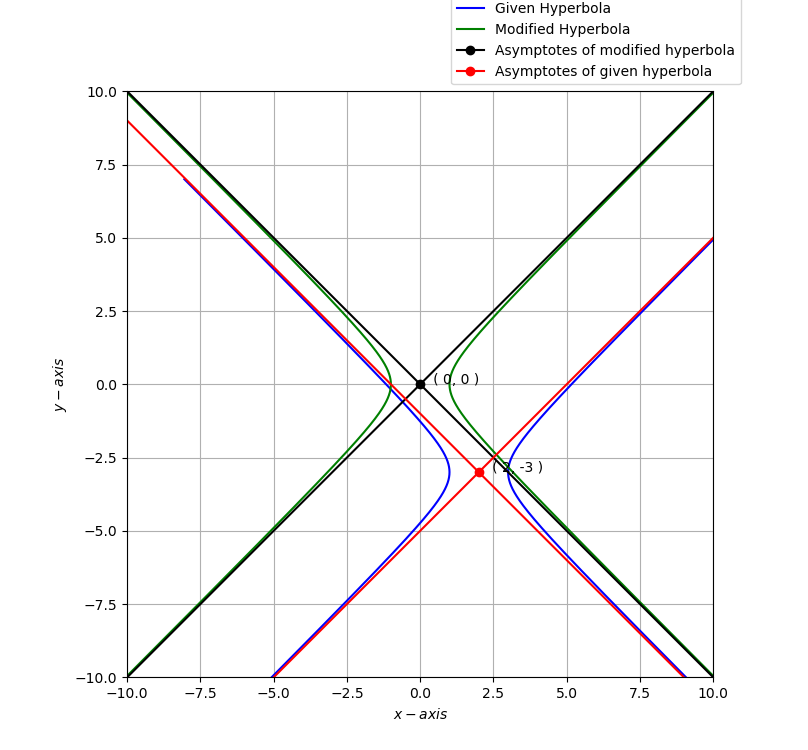
\includegraphics[width=11cm]{Figure_1.png}
    \caption{Plot of the Asymtotes.}
    \label{Plot of the Asymtotes}
\end{figure}
\end{document}